\mySection{9.1 Introduction}
%-------------- start slide -------------------------------%{{{ 9.4
\begin{frame}
\begin{center}
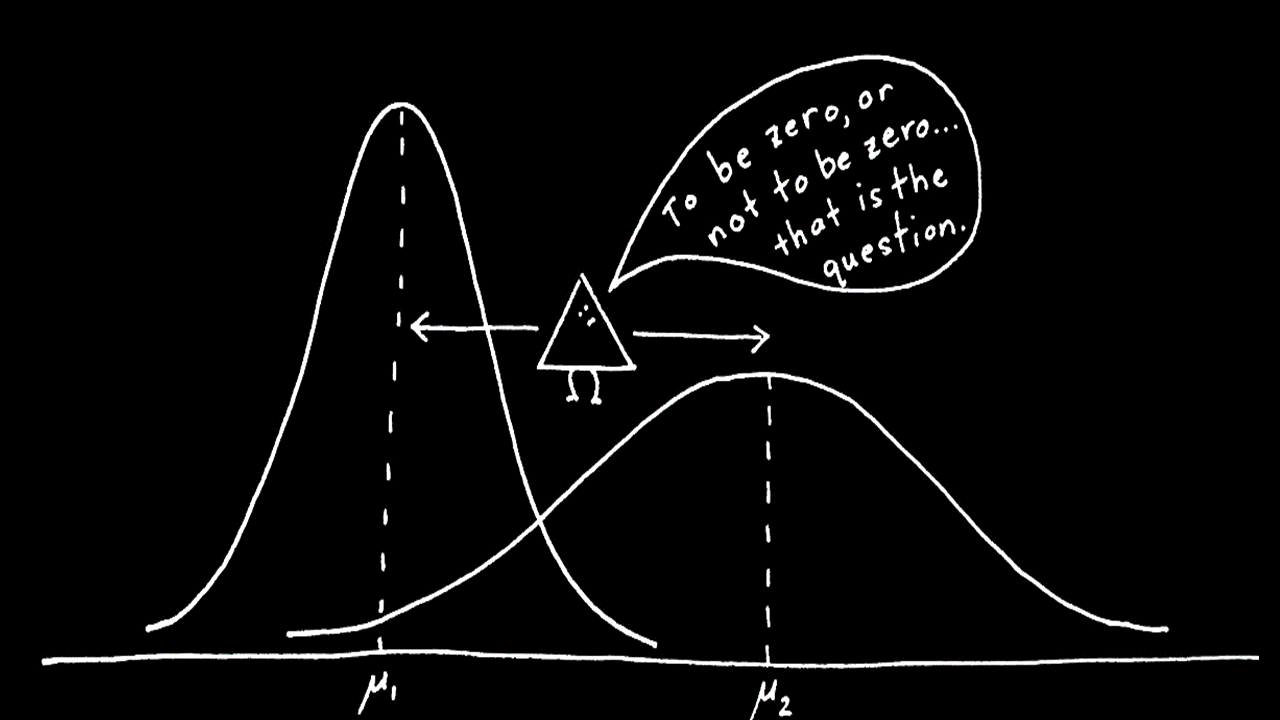
\includegraphics[scale=0.18]{TwoSample_Test-neg.png}\\
\end{center}
\pause
Multilevel designs:\\[1em]

\begin{enumerate}
\item Two methods applied to two independent sets of similar subjects.\\[1em]
E.g., comparing two products.
\vfill
\item Same method applied to two different kinds of subjects. \\[1em]
E.g., comparing bones of European kids and American kids.
\end{enumerate}
\end{frame}
%-------------- end slide -------------------------------%}}}
%-------------- start slide -------------------------------%{{{ 9.5
\begin{frame}{Test for normal parameters (two sample test)}
\begin{enumerate}
\item Let $X_1,\cdots, X_n$ be a random sample of size $n$ from $N(\mu_X,\sigma^2_X)$.	\\[1em]
\item Let $Y_1,\cdots, Y_m$ be a random sample of size $m$ from $N(\mu_Y,\sigma^2_Y)$.
\vfill
\item[Prob. 1] Find a test statistic $\Lambda$ in order to test\hfill $H_0 : \mu_X = \mu_Y$ v.s. $H_1 : \mu_X \ne \mu_Y$. \\[2em]
\item[1-1]When $\sigma^2_X$ and $\sigma^2_Y$ are known\\[1em]
\item[1-2]When $\sigma^2_X = \sigma^2_Y$ is unknown\\[1em]
\item[1-3]When $\sigma^2_X \ne \sigma^2_Y$, both are unknown
\pause \hspace{3em}
\vfill
\item[Prob. 2] Find a test statistic $\Lambda$ in order to test\hfill $H_0 : \sigma_X^2 = \sigma_Y^2$ v.s. $H_1 : \sigma_X^2 \ne \sigma^2_Y$. \\[2em]
\end{enumerate}
\end{frame}
%-------------- end slide -------------------------------%}}}
%-------------- start slide -------------------------------%{{{ 9.6
\begin{frame}
\begin{enumerate}
	\item[Prob. 1-1] Find a test statistic for $H_0 : \mu_X = \mu_Y$ v.s. $H_1 : \mu_X \ne \mu_Y$, \\[1em]
	with $\sigma^2_X$ and $\sigma^2_Y$ known.\\[2em]
	\vfill
	\item[Sol.]
	\[
		\frac{\overline{X}-\overline{Y}-(\mu_X-\mu_Y)}{\sqrt{\frac{\sigma_X^2}{n}+\frac{\sigma_Y^2}{m} }} =
		\frac{\overline{X}-\overline{Y}}{\sqrt{\frac{\sigma_X^2}{n}+\frac{\sigma_Y^2}{m} }} \sim N(0,1)
	\]
	\vfill
	\item[] Test statistics: $z = \frac{\bar{x}-\bar{y}}{\sqrt{\frac{\sigma_X^2}{n}+\frac{\sigma_Y^2}{m} }}$.
	\vfill
	\item[] Critical region $|z|\ge z_{\alpha/2}$. \myEnd
\end{enumerate}
\end{frame}
%-------------- end slide -------------------------------%}}}
%-------------- start slide -------------------------------%{{{ 9.7
\begin{frame}
\begin{enumerate}
	\item[Prob. 1-2] Find a test statistic for $H_0 : \mu_X = \mu_Y$ v.s. $H_1 : \mu_X \ne \mu_Y$, \\[1em]
		with $\sigma^2_X = \sigma^2_Y=\sigma^2$ but unknown.\\[2em]
\vfill
\item[Sol.] Composite-vs-composite test with:
\[\omega =\left\{(\mu_X,\mu_Y,\sigma^2): \mu_X=\mu_Y\in\R, \hspace{1.4em} \sigma^2>0\right\}\]
\[\Omega =\left\{(\mu_X,\mu_Y,\sigma^2): \mu_X\in\R,\: \mu_Y\in\R, \: \sigma^2>0\right\}\]\\[2em]
\item[] The likelihood function
	\begin{align*}
		L(\omega)= & \prod_{i=1}^n f_X(x_i) \prod_{j=1}^mf_Y(y_j)\\[2em]
		=&\left(  \frac{1}{\sqrt{2\pi}\:\sigma} \right)^{m+n}\exp \left(
	- \frac{1}{2\sigma^2} \left[\sum_{i=1}^n (x_i-\mu_X)^2 + \sum_{j=1}^m (y_i-\mu_Y)^2
	\right]
\right)
	\end{align*}
\end{enumerate}
\end{frame}
%-------------- end slide -------------------------------%}}}
%-------------- start slide -------------------------------%{{{ 9.8
\begin{frame}
	\begin{enumerate}
		\item[] Under $\omega$, the MLE $\omega_e=(\mu_{\omega_e},\mu_{\omega_e},\sigma_{\omega_e}^2)$ is\\[1em]
\begin{align*}
	\mu_{\omega_e} &=  \frac{\sum_{i=1}^n x_i+\sum_{j=1}^m y_j}{n+m}\\[2em]
	\sigma_{\omega_e}^2 &=   \frac{\sum_{i=1}^n (x_i-\mu_{\omega_e})^2+\sum_{j=1}^m (y_j-\mu_{\omega_e})^2}{n+m}
\end{align*}
\vfill
\item[] Hence,
	\[
		L(\omega_e) = \left(  \frac{e^{-1}}{2\pi\sigma_{\omega_e}^2}\right)^{ \frac{n+m}{2}}
	\]
	\end{enumerate}
\end{frame}
%-------------- end slide -------------------------------%}}}
%-------------- start slide -------------------------------%{{{ 9.9
\begin{frame}

	\begin{enumerate}
		\item[] Under $\Omega$, the MLE $\omega_e=(\mu_{X_e},\mu_{Y_e},\sigma_{\Omega_e}^2)$ is\\[1em]
			\[
				\mu_{X_e} =\frac{1}{n} \sum_{i=1}^{n}x_i \quad\text{and}\quad \mu_{Y_e}=\frac{1}{m} \sum_{j=1}^{m}y_j
			\]
			\\[1em]
			\[
				\sigma_{\Omega_e}^2 =
	 \frac{\sum_{i=1}^n (x_i-\mu_{X_e})^2+\sum_{j=1}^m (y_j-\mu_{Y_e})^2}{n+m}
			\]
			\vfill
		\item[] Hence,
			\[
				L(\Omega_e)
		= \left(  \frac{e^{-1}}{2\pi\sigma_{\Omega_e}^2}\right)^{ \frac{n+m}{2}}
			\]
	\end{enumerate}
\end{frame}
%-------------- end slide -------------------------------%}}}
%-------------- start slide -------------------------------%{{{ 9.10
\begin{frame}

	\begin{enumerate}
		\item[]
			\[
				\lambda =  \frac{L(\omega_e)}{L(\Omega_e)}= \left(  \frac{\sigma^2_{\Omega_e}}{\sigma^2_{\omega_e}}\right)^{ \frac{m+n}{2}}
			\]
			\vfill
\[
\lambda^{ \frac{2}{n+m}} =  \frac{\sum_{i=1}^n (x_i-\bar{x})^2+\sum_{j=1}^n (y_j-\bar{y})^2}{\sum_{i=1}^n \left(x_i- \frac{n\bar{x}+m\bar{y}}{m+n}\right)^2+\sum_{j=1}^n \left(y_j-\frac{n\bar{x}+m\bar{y}}{m+n}\right)^2}
\]
	\end{enumerate}
\end{frame}
%-------------- end slide -------------------------------%}}}
%-------------- start slide -------------------------------%{{{ 9.11
\begin{frame}
\begin{enumerate}
	\item []
		\begin{align*}
		\sum_{i=1}^n \left(x_i- \frac{n\bar{x}+m\bar{y}}{m+n}\right)^2 = \sum_{i=1}^n (x_i-\bar{x})^2 +  \frac{m^2n}{(m+n)^2} (\bar{x}-\bar{y})^2
		\end{align*}
		\vfill
		\begin{align*}
		\sum_{j=1}^m \left(y_j- \frac{n\bar{x}+m\bar{y}}{m+n}\right)^2 = \sum_{j=1}^m (y_i-\bar{y})^2 +  \frac{mn^2}{(m+n)^2} (\bar{x}-\bar{y})^2
	\end{align*}
		\vfill
	\item[]
		\begin{align*}
			\Downarrow
		\end{align*}
		\begin{gather*}
			\sum_{i=1}^n \left(x_i- \frac{n\bar{x}+m\bar{y}}{m+n}\right)^2+ \sum_{j=1}^n \left(y_j-\frac{n\bar{x}+m\bar{y}}{m+n}\right)^2 \\
				 || \\
			\sum_{i=1}^n (x_i-\bar{x})^2 + \sum_{j=1}^m (y_i-\bar{y})^2+  \frac{mn}{m+n} (\bar{x}-\bar{y})^2
		\end{gather*}
\end{enumerate}
\end{frame}
%-------------- end slide -------------------------------%}}}
%-------------- start slide -------------------------------%{{{ 9.12
\begin{frame}
	\begin{align*}
		\lambda^{ \frac{2}{m+n}} &=
		\frac{\sum_{i=1}^n (x_i-\bar{x})^2 + \sum_{j=1}^m (y_i-\bar{y})^2}{\sum_{i=1}^n (x_i-\bar{x})^2 + \sum_{j=1}^m (y_i-\bar{y})^2+  \frac{mn}{m+n}(\bar{x}-\bar{y})^2}\\[1em]
& =  \frac{1}{\displaystyle 1+  \frac{(\bar{x}-\bar{y})^2}{  \left[ \sum_{i=1}^n (x_i-\bar{x})^2 + \sum_{j=1}^m (y_i-\bar{y})^2 \right] \left( \frac{1}{m} + \frac{1}{n}  \right)}}
		\\[2em]& =  \frac{n+m-2}{\displaystyle n+m-2+  \frac{(\bar{x}-\bar{y})^2}{ \alert{ \frac{1}{n+m-2} \left[ \sum_{i=1}^n (x_i-\bar{x})^2 + \sum_{j=1}^m (y_i-\bar{y})^2 \right]} \left( \frac{1}{m} + \frac{1}{n}  \right)}}
		\\[2em] &=
		\frac{n+m-2}{\displaystyle n+m-2 +  \frac{(\bar{x}-\bar{y})^2}{\alert{s_p^2}\left(  \frac{1}{m}+  \frac{1}{n}\right)}}
		 =
		\frac{n+m-2}{n+m-2+t^2}.
	\end{align*}
	\vfill	\[
	\boxed{t :=  \frac{\bar{x}-\bar{y}}{s_p\sqrt{  \frac{1}{m}+  \frac{1}{n}} }}
	\]
\end{frame}
%-------------- end slide -------------------------------%}}}
%-------------- start slide -------------------------------%{{{ 9.13
\begin{frame}
\centering
\[
	t\mapsto  \frac{a}{a+t^2}
\]
\vfill
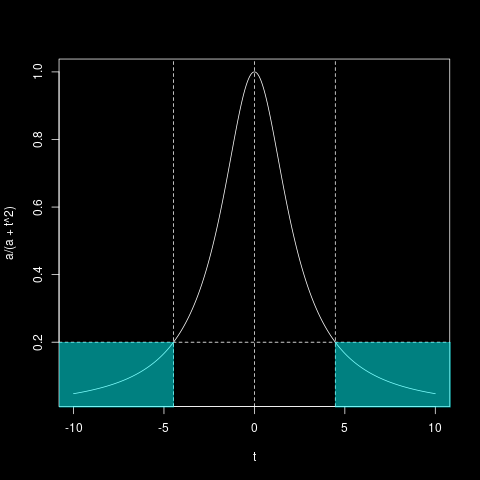
\includegraphics[scale=0.4]{T-Statistics-neg.png}
\end{frame}
%-------------- end slide -------------------------------%}}}
%-------------- start slide -------------------------------%{{{ 9.14
\begin{frame}

	\begin{enumerate}
		\item[] One can use the following statistic \\[1em]
			\[
				T =  \frac{\overline{X}-\overline{Y}}{S_p \sqrt{ \frac{1}{m}+ \frac{1}{n} }}
			\]
			\vfill
		\item[] where $S_p^2$ is called the \textcolor{yellow!80!black}{\it pooled sample variance}\\[1em]
			\begin{align*}
				S_p^2 =&  \frac{1}{n+m-2}\left[  \textcolor{magenta}{\sum_{i=1}^n \left(X_i -\overline{X} \right )^2}+ \textcolor{blue}{\sum_{i=1}^m \left(Y_j -\overline{Y} \right )^2}\right ]
				\\[1em] =&  \frac{1}{n+m-2}\left[ \textcolor{magenta}{(n-1)S_X^2} + \textcolor{blue}{(m-1) S_Y^2} \right ]
			\end{align*}
	\end{enumerate}
\end{frame}
%-------------- end slide -------------------------------%}}}
%-------------- start slide -------------------------------%{{{ 9.15
\begin{frame}
Three observations:
\vfill
	\begin{enumerate}
		\item $\E[\overline{X}-\overline{Y}] = 0$ and
			\[
\Var(\overline{X}-\overline{Y}) =
\Var(\overline{X})+ \Var(\overline{Y})
=  \frac{\sigma_X^2}{n} +  \frac{\sigma_Y^2}{m}
= \sigma^2 \left(  \frac{1}{n}+  \frac{1}{m}\right)
\]
\item[] Hence, $\textcolor{yellow}{\frac{\overline{X}-\overline{Y}}{\sigma\sqrt{\frac 1n + \frac 1m}}}\sim N(0,1)$
\vfill
\item $\textcolor{red}{\frac{n+m-2}{\sigma^2} S_p^2} = \sum_{i=1}^n \left(\frac{X_i-\overline{X}}{\sigma}\right)^2
	+ \sum_{j=1}^m \left(\frac{Y_j-\overline{Y}}{\sigma}\right)^2 \sim $ Chi square$(n+m-2)$
	\vfill
\item $\textcolor{yellow}{\frac{\overline{X}-\overline{Y}}{\sigma\sqrt{\frac 1n + \frac 1m}}} \perp  \textcolor{red}{\frac{n+m-2}{\sigma^2}S_p^2}$
	\vfill
\item[$\Longrightarrow$] $T = \frac{\displaystyle\textcolor{yellow}{\frac{\overline{X}-\overline{Y}}{\sigma\sqrt{\frac 1n+\frac 1m}}} }{\displaystyle\sqrt{\textcolor{red}{\frac{n+m-2}{\sigma^2} S_p^2}\times \frac{1}{n+m-2} }} = \frac{\overline{X}-\overline{Y}}{S_p \sqrt{ \frac{1}{m}+ \frac{1}{n} }} \sim $ t distr.$(n+m-2)$
	\end{enumerate}
\end{frame}
%-------------- end slide -------------------------------%}}}
%-------------- start slide -------------------------------%{{{ 9.16
\begin{frame}
	Finally, \\[2em]
\begin{enumerate}
	\item[] Test statistics: $t= \frac{\bar{x}-\bar{y}}{s_p\sqrt{\frac1m+\frac1n}}$
		\vfill
	\item[] Critical region: $|t|\ge t_{\alpha/2,n+m-2}$. \myEnd
\end{enumerate}
\end{frame}
%-------------- end slide -------------------------------%}}}
%-------------- start slide -------------------------------%{{{ 9.17
\begin{frame}
\begin{enumerate}
	\item[Prob. 1-3] Find a test statistic for $H_0 : \mu_X = \mu_Y$ v.s. $H_1 : \mu_X \ne \mu_Y$, \\[1em]
		with $\sigma^2_X \ne \sigma^2_Y$, both unknown.\\[2em]
		\vfill
	\item[Remark:] 1. Known as the {\it \textcolor{yellow}{Behrens-Fisher problem}}.
			\vfill
		\item[] 2. No exact solutions!
			\vfill
		\item[] 3. We will derive a widely used approximation by
			\vspace{3em}
			% \\[2em]
		\item[]	\hspace{5em} {\it Bernard Lewis Welch} (1911--1989)
\end{enumerate}

\end{frame}
%-------------- end slide -------------------------------%}}}
%-------------- start slide -------------------------------%{{{ 9.18
\begin{frame}

	\begin{enumerate}
		\item[Sol.]
	\[
W =  \frac{\overline{X}-\overline{Y}-(\mu_X-\mu_Y)}{\sqrt{ \frac{S^2_X}{n}+\frac{S^2_Y}{m}  }}
=  \frac{\overline{X}-\overline{Y}-(\mu_X-\mu_Y)}{\sqrt{ \frac{\sigma^2_X}{n}+\frac{\sigma^2_Y}{m}  }}
\Bigg/  \frac{\sqrt{ \frac{S^2_X}{n}+\frac{S^2_Y}{m}  }}{\sqrt{ \frac{\sigma^2_X}{n}+\frac{\sigma^2_Y}{ m} }}
\]
\vfill \item[]
\[
U:=\frac{\overline{X}-\overline{Y}-(\mu_X-\mu_Y)}{\sqrt{ \frac{\sigma^2_X}{n}+\frac{\sigma^2_Y}{m} }}\sim N(0,1)
\]
\vfill
\item[]
\[
\frac{V}{\nu}:= \frac{\displaystyle\frac{S^2_X}{n}+\frac{S^2_Y}{m}}{\displaystyle\frac{\sigma^2_X}{n}+\frac{\sigma^2_Y}{m}}
\]
	\end{enumerate}
\end{frame}
%-------------- end slide -------------------------------%}}}
%-------------- start slide -------------------------------%{{{ 9.19
\begin{frame}
\begin{itemize}
	\item[!!] {\bf Assumption/Approximation:} \\[1em]
		Assume that $V$ follows Chi Square$(\nu)$ and assume that $V\perp U$.
	\vfill
\item[$\Longrightarrow$] Then, $W\sim$ Student's t-distribution of freedom $\nu$.
	\vfill
\item[?] It remains to estimate $\nu$: Suppose we have
\[
\nu= \frac{\left(  \frac{\sigma_X^2}{n}+ \frac{\sigma_Y^2}{m} \right)^2 }
{ \frac{\sigma_X^4}{n^2(n-1)}+\frac{\sigma_Y^4}{m^2(m-1) }}
=
\frac{\left(\theta+ \frac{n}{m} \right)^2}{ \frac{1}{n-1}\theta^2 +  \frac{1}{m-1}\left(  \frac{n}{m}\right)^2},
\quad \theta= \frac{\sigma_X^2}{\sigma_Y^2}.
\]
\vfill
\item[!!] Still need to know $\theta = \sigma_X^2/\sigma_Y^2$... Another approximation $\hat\theta=S_X^2/S_Y^2$, i.e., \\[1em]
\[
\nu \approx
\frac{\left(\frac{s_X^2}{n}+ \frac{s_Y^2}{m} \right)^2 }
{ \frac{s_X^4}{n^2(n-1)}+\frac{s_Y^4}{m^2(m-1) }}
=  \frac{\left(\hat\theta+ \frac{n}{m} \right)^2}{ \frac{1}{n-1}\hat\theta^2 +  \frac{1}{m-1}\left(  \frac{n}{m}\right)^2},
\quad \hat\theta= \frac{s_X^2}{s_Y^2}.
\]
\end{itemize}

\end{frame}
%-------------- end slide -------------------------------%}}}
%-------------- start slide -------------------------------%{{{ 9.20
\begin{frame}

\begin{enumerate}
	\item[] In summary: \\[1em]
		\[
			W =  \frac{\overline{X}-\overline{Y}-(\mu_X-\mu_Y)}{\sqrt{ \frac{S^2_X}{n}+\frac{S^2_Y}{m} }}
			\sim \text{Student's t of freedom $\nu$}
		\]
\vfill
\item[]
\[
	\nu  = \left[
\frac{\left(\frac{s_X^2}{n}+ \frac{s_Y^2}{m} \right)^2 }
{ \frac{s_X^4}{n^2(n-1)}+\frac{s_Y^4}{m^2(m-1) }}
	\right]
	=
	\left[
\frac{\left(\hat\theta+ \frac{n}{m} \right)^2}{ \frac{1}{n-1}\hat\theta^2 +  \frac{1}{m-1}\left(  \frac{n}{m}\right)^2}
	\right],
\quad \hat\theta= \frac{s_X^2}{s_Y^2}.
\]
\vfill
\item[] Test statistic: $t = \frac{\bar{x}-\bar{y}-(\mu_X-\mu_Y)}{\sqrt{ \frac{s^2_X}{n}+\frac{s^2_Y}{m} }}
$
\vfill
\item[] Critical region: $|t|\ge t_{\alpha/2,\nu}$.\myEnd
	\vfill
\item[Remark] If $\nu \ge 100$, replace the t-score, e.g., $t_{\alpha/2,\nu}$ by the z-score, e.g., $z_{\alpha/2}$.
	\end{enumerate}
\end{frame}
%-------------- end slide -------------------------------%}}}
%-------------- start slide -------------------------------%{{{ 9.21
\begin{frame}

	\begin{enumerate}
		\item[Thm ] The moment estimate for $\nu$
			\begin{align*}
	\nu &=   \frac{\left(  \frac{\sigma_X^2}{n}+ \frac{\sigma_Y^2}{m} \right)^2 }
{ \frac{\sigma_X^4}{n^2(n-1)}+\frac{\sigma_Y^4}{m^2(m-1) }+ \frac{\sigma_X^2\sigma_Y^2}{mn}}
	\\[2em] & \approx
\frac{\left(  \frac{\sigma_X^2}{n}+ \frac{\sigma_Y^2}{m} \right)^2 }
{ \frac{\sigma_X^4}{n^2(n-1)}+\frac{\sigma_Y^4}{m^2(m-1) }}
=
\frac{\left(\theta+ \frac{n}{m} \right)^2}{ \frac{1}{n-1}\theta^2 +  \frac{1}{m-1}\left(  \frac{n}{m}\right)^2},
\quad \theta= \frac{\sigma_X^2}{\sigma_Y^2}.
			\end{align*}
\vfill
\item[Proof.]
\[
	\frac{V}{\nu}\left( \frac{\sigma^2_X}{n}+\frac{\sigma^2_Y}{m} \right)= \frac{S^2_X}{n}+\frac{S^2_Y}{m}
\]
\vfill
\item[]$(n-1)S_X^2/\sigma_X^2\sim$ Chi Sqr$(n-1) \Longrightarrow\E(S_X^2)= \sigma_X^2$. Similarly, $\E(S_Y^2)= \sigma_Y^2$.
	\end{enumerate}
\end{frame}
%-------------- end slide -------------------------------%}}}
%-------------- start slide -------------------------------%{{{ 9.22
\begin{frame}

	\begin{enumerate}
\item[] First moment gives identity. Need to consider second moment.
\item[] Second moments for Chi sqr(r) is $2r$. Hence, $\E(S_X^4) =  \frac{\sigma_X^4}{n-1}$.
\item[]
			\begin{align*}
			 \frac{2\nu}{\nu^2}
	\left( \frac{\sigma^2_X}{n}+\frac{\sigma^2_Y}{m} \right)^2
	&= 2\frac{\sigma^4_X}{n^2(n-1)}+2\frac{\sigma^4_Y}{m^2(m-1)}
	+  2\frac{\sigma_X^2\sigma_Y^2}{mn}
				% \\[2em]&\approx 2\frac{\sigma^4_X}{n^2(n-1)}+2\frac{\sigma^4_Y}{m^2(m-1)}
			\end{align*}
		\item[] ... \myEnd
			\vfill
	\item[Remark] Welch (1938) approximation is more involved, which actually assumes that $V$ follows the {\it Type III Pearson distribution}.
	\item[]	\url{https://en.wikipedia.org/wiki/Behrens-Fisher_problem}
	\end{enumerate}
\end{frame}
%-------------- end slide -------------------------------%}}}
%-------------- start slide -------------------------------%{{{ 9.23
\begin{frame}
	\begin{enumerate}
		\item[Prob. 2] Find a test statistic $\Lambda$ in order to test\qquad $H_0 : \sigma_X^2 = \sigma_Y^2$ v.s. $H_1 : \sigma_X^2 \ne \sigma^2_Y$. \\[2em]
		\vfill
		\item[Sol.]
			\[
			\frac{S_X^2/\sigma_X^2}{S_Y^2/\sigma_Y^2} \sim \text{F-disribution $(n-1,m-1)$}
			\]
			\vfill
		\item[] Test statistic: $f =\frac{s_X^2/\sigma_X^2}{s_Y^2/\sigma_Y^2}=\frac{s_X^2}{s_Y^2} $
			\vfill
		\item[] Critical regions: $f\le  F_{\alpha/2,n-1,m-1}$ or $f\ge F_{1-\alpha/2,n-1,m-1}$. \myEnd
	\end{enumerate}
\end{frame}
%-------------- end slide -------------------------------%}}}
